\chapter{Simulation}
In our work, we have created a knowledge base that can infer parameters to enable an agent to perform various actions.
Since testing these actions on a real robot proves to be challenging, we do so in a simulation.
This chapter aims to provide an overview of the \nameref{sec:simulation environment} in which we test our work and present it as a proof of concept.
Initially, we will explain the environment, including objects, followed by an overview of the motion primitives.
Finally, we will showcase some of our motions (in \nameref{sec:simulated motions}) and discuss the \nameref{sec: simulation to real world gap} before drawing a conclusion where we discuss existing challenges.

\section{Simulation Environment}
\label{sec:simulation environment}

We utilize the simulation environment \textit{BulletWorld}, which is already integrated into the framework \textit{PyCRAM} \hyperref[sec:pycram]{(PyCRAM)}. In this environment, physics is simulated, which is advantageous for executing the motions we have defined or customized. Additionally, leveraging the \textit{PyCRAM} framework allows us to utilize various existing control primitives, such as \textit{Pick and Place}. Communication between the simulation and framework is facilitated by \textit{ROS1} \hyperref[sec:ROS]{(ROS)}, which communicates via various nodes, each representing a joint, for instance. Through these nodes, one can obtain information about the joints or transmit commands to modify the parameters of the joints accordingly.


The agent that will execute the various motions in the simulation is the  \textit{PR2} \hyperref[sec:pr2]{(PR2)}.
This robot model has 2 movable arms, which is important for our work, as one hand executes the motion while the other arm holds the container in which the action is performed. In addition to the fact that the \textit{PR2} model is already available in the \textit{PyCram} framework,
the \textit{PR2} model also has enough joints and degrees of freedom to execute the motions we have adapted.

The agent operates in a kitchen-like environment, the model of which is already included in the \textit{PyCRAM}-core and therefore particularly suitable for our use case. The kitchen also features elements such as drawers that can be opened, indicating an approximation to a real kitchen. Additionally, the kitchen model includes a table on which the agent's actions are ultimately executed. Other furniture is also present in this environment, but is not relevant to our use case.

\begin{figure}[H]
    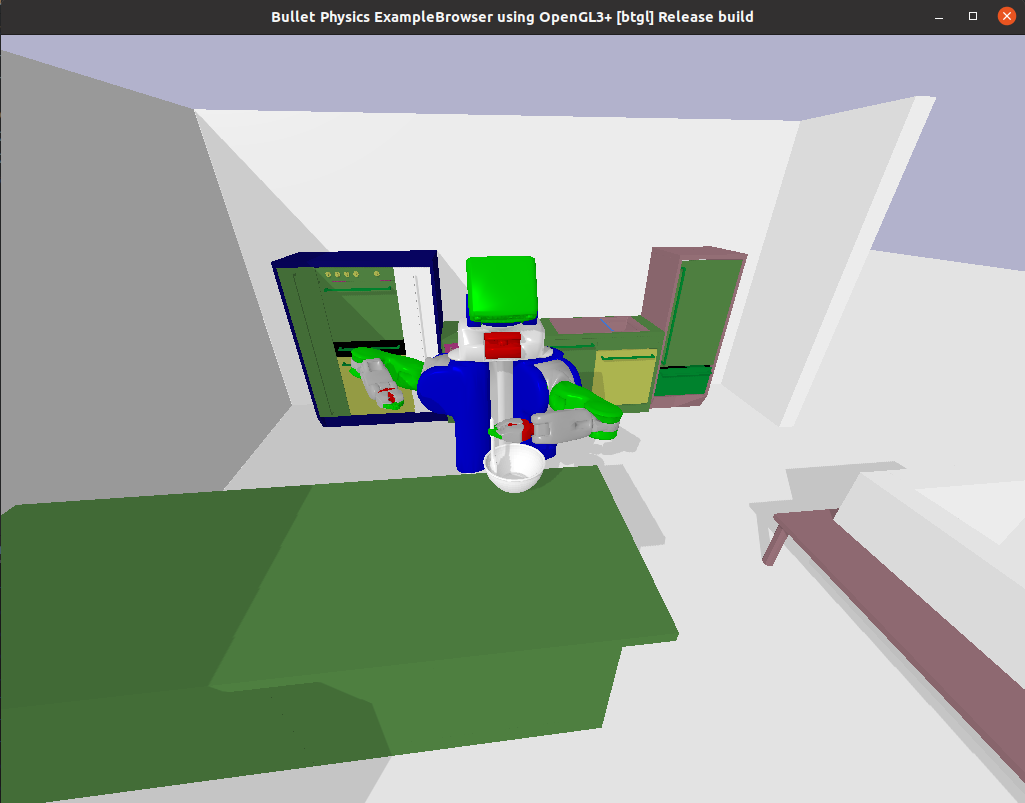
\includegraphics[scale=0.35]{Graphics/bulletworldexample.png}
    \label{fig:bulletworldexample}
    \caption{Simulation Environment containing the \textit{PR2} and \textit{Kitchen} models. }
\end{figure}

For the simulation, we use the objects that have also been defined in the ontology (see \hyperref[sec:ContainersAndToolsAcquisition]{Containers and Tools Acquisition}).
The following objects are available:
\begin{itemize}
	\item Container: small and large bowls (defined in the ontology as \textit{SaladBowl} and \textit{PastaBowl}), pan, pot, cup, and mug.
	\item Tools: whisk (even though it is not defined in the ontology, we still use it as it is a very commonly used mixing instrument), spoon, wooden spoon, and fork.
\end{itemize}

\begin{figure}[H]
    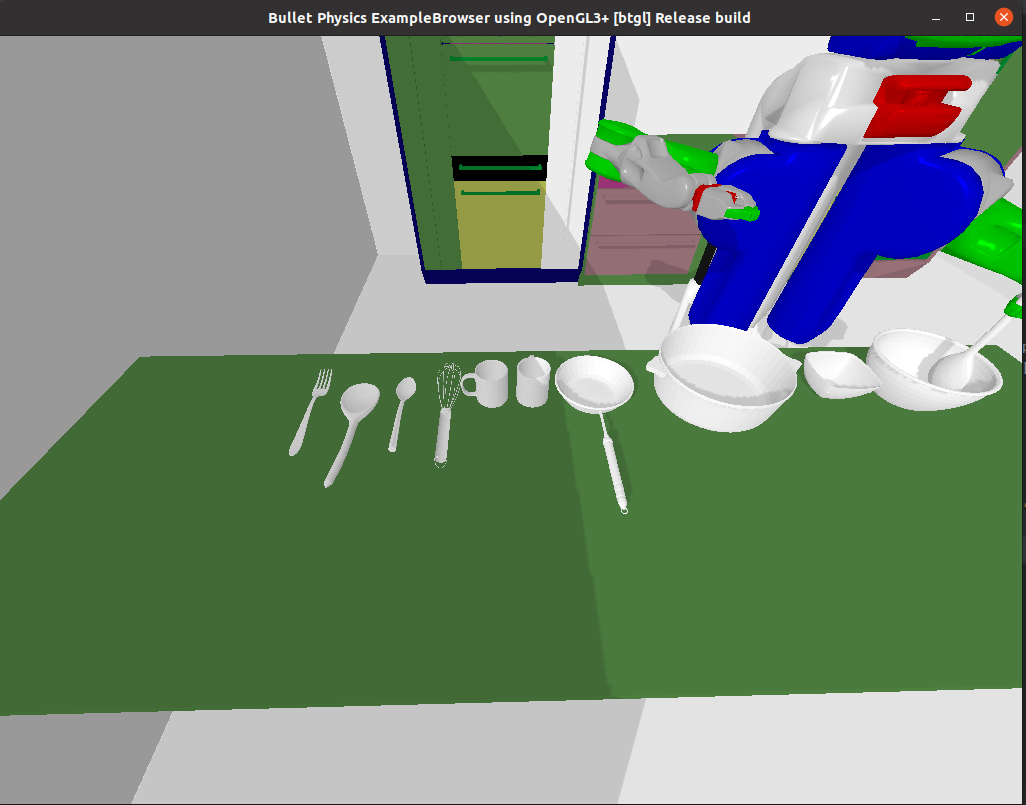
\includegraphics[scale=0.35]{Graphics/toolscontainersmodels.png}
    \label{fig:toolscontainersmodels}
    \caption{Used models for the simulation: \textit{Fork, WoodenSpoon, Spoon, Whisk, Mug, Cup, Pan, Pot, Small Bowl, Big Bowl}}
\end{figure}

In the simulation itself, there are no ingredients. When executing the motion, we assume a set of given ingredients, which ultimately play a role in selecting the parameters (see \hyperref[chap:Data_representation]{Data Representation}). Representing ingredients in a simulation proves to be challenging, in addition to the fact that modeling the creation of the mixed ingredients would also be necessary. This approach is also addressed in the section \nameref*{sec:Future Work} (REFERENCE FUTURE WORK).

\section{Control Primitives}
The framework \nameref{sec:pycram} offers a variety of pre-implemented control primitives. These primitives can be used as building blocks to structure the entire execution of a task. These primitives are also defined as \textit{Action Designators}, and the following ones are relevant for our use case:

\begin{lstlisting}
	NavigateAction(target_locations=[pickup_pose.pose]).
					resolve().perform()
\end{lstlisting}

\newpage

\begin{lstlisting}
	PickUpAction(object_designator_description=tool_object,
                 arms=pickup_pose.reachable_arms,
                 grasps=["top"]).resolve().perform()
\end{lstlisting}

\begin{lstlisting}
	NavigateAction(target_locations=[nav_pose]).
					resolve().perform()
\end{lstlisting}

\begin{lstlisting}
	LookAtAction(targets=[container_object.resolve().pose]).
					resolve().perform()
\end{lstlisting}

\begin{lstlisting}
	MixingActionSWRL(
		object_designator_description=container_object,
        object_tool_designator_description=tool_object,
		ingredients=[Set of Ingredients],
        task="given task",
        arms=["left"],
        grasps=["top"]).parameters_from_owl().perform()
\end{lstlisting}

The last \textit{Action Designator} is a modified version of the existing \textit{Mixing Action Designator}, which has been adapted for our purposes. This designator receives as parameters a container object and a tool object (both not significant for inference), as well as a set of ingredients and a task, which are significant for inference. The performed motion results from the inference together with the applied parameters (HERE POINT OUT TO SOMETHING).

\begin{figure}[H]
    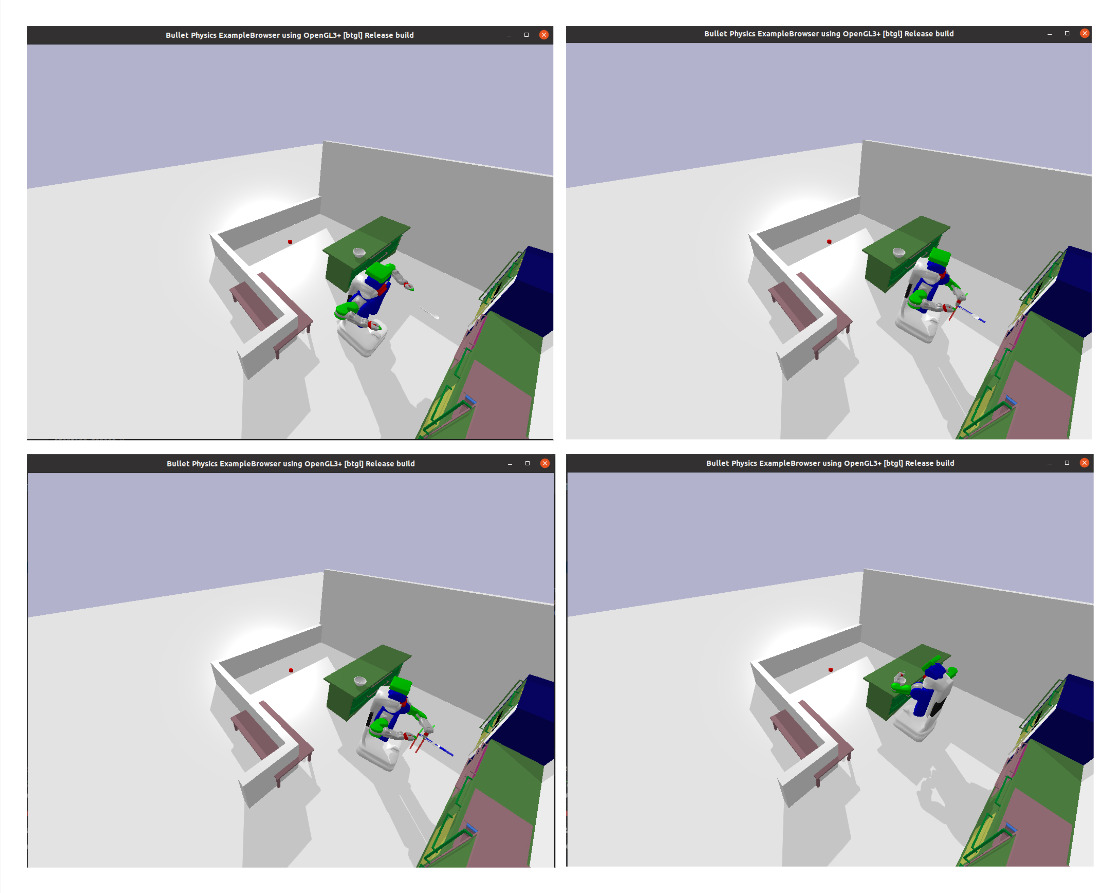
\includegraphics[scale=0.3]{Graphics/control_primitives.jpg}
    \label{fig:controlprimitives}
    \caption{Feautured \textit{Control Primitives}}
\end{figure}


\section{Simulated Motions}
\label{sec:simulated motions}
In this section, we aim to illustrate how the motions we have implemented.
We will discuss the respective movements as well as the parameters involved. In \nameref{sec:pycram}, there is the option to interpret the motions as visual axes, which simulate the process of the executed motion beforehand. In this section, we therefore showcase the various motions as they appear in the simulation with these axes, along with a sketch of the implemented movements.



\subsection{Whirlstorm Motion}
The Whirlstorm motion was already an implemented motion in \nameref{sec:pycram}. In our version, we have slightly modified the motion (see Chapter \nameref{chap:Motions}).

\begin{figure}[H]
    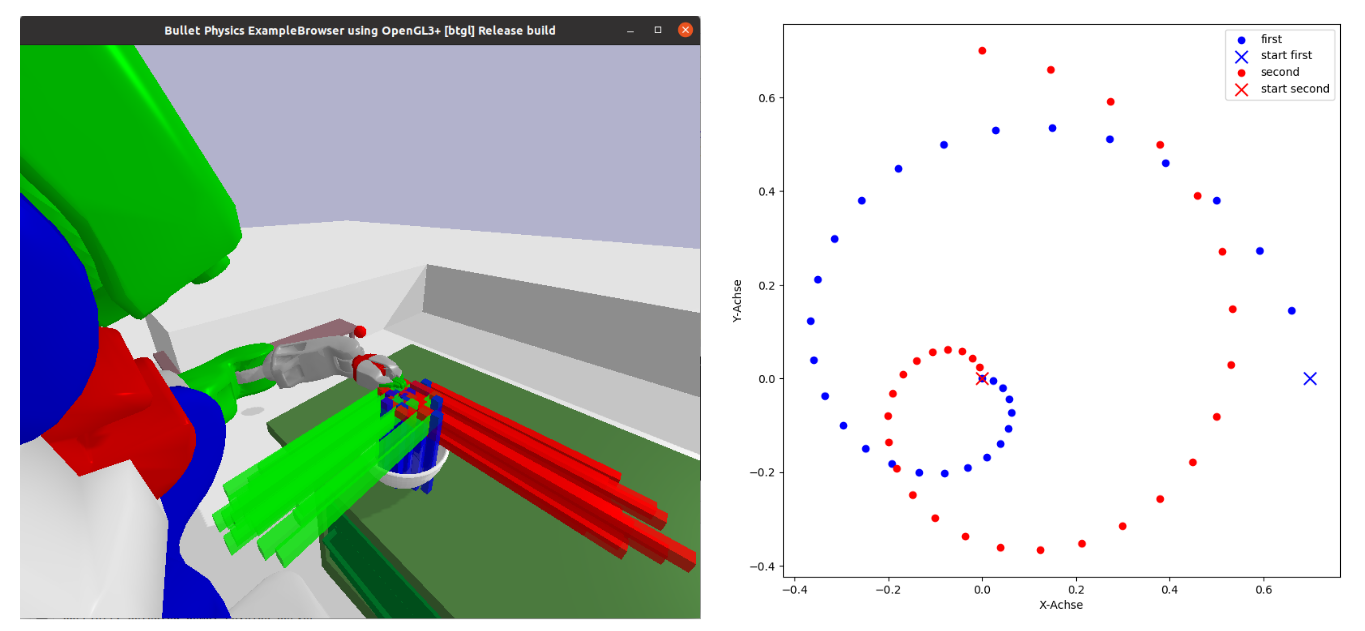
\includegraphics[scale=0.3]{Graphics/whirlstormshowcase.png}
    \label{fig:whirlstormshowcase}
    \caption{Feautured \textit{Whirlstorm Motion}}
\end{figure}

In Figure \ref{fig:whirlstormshowcase}, it can be observed that the Whirlstorm motion has two starting points. Initially, the motion starts at the edge of the container and then moves counterclockwise to the second starting point, from which the motion continues analogously.

\subsection{Circular Motion}
Same as above
\subsection{Vertical Circular Motion}
Same as above
\subsection{Folding Motion}
Same as above

\section{Simulation to Real-World gap}
\label{sec: simulation to real world gap}

In a kitchen setting, a robot faces many challenges when it comes to MixingMotion, especially in the real world compared to a simulation.
Unlike simulations where movements are precise and predictable, real-world scenarios throw unexpected obstacles, different surface textures, and possible interruptions from human interactions at the robot.
Additionally, environmental factors can affect the robot's sensors, leading to misinterpretations or inaccurate readings.
Dealing with the complexity and unpredictability of a real kitchen environment requires sophisticated planning and control algorithms that go beyond relying solely on simulation data.

When it comes to mixing various ingredients in the real world as opposed to a simulation, several factors can go awry. Firstly, the physical properties of ingredients can vary widely, such as viscosity, density, and texture, which may not be accurately represented in a simulation.
This can lead to unexpected interactions between ingredients, resulting in inconsistent mixing patterns or clumping. Additionally, the dynamics of the mixing process may be influenced by external factors such as temperature variations, air currents, and uneven distribution of ingredients within the mixing vessel, all of which are challenging to simulate accurately.
Moreover, the mechanical limitations of the robot, such as its speed, precision, and ability to adapt to changing conditions, can further complicate the mixing process in the real world.
These discrepancies between simulation and reality highlight the need for robust control strategies that can adapt to the complexities of real-world mixing scenarios.

From a perception standpoint, uncertainty in the real world during mixing tasks can stem from various sources.
One significant factor is the limited accuracy and reliability of sensors in capturing detailed information about the environment and the ingredients being mixed.
Lighting conditions, reflections, and occlusions can obscure the robot's view, leading to incomplete or distorted perception of the mixing process.
Additionally, the inherent variability in appearance and shape of ingredients can pose challenges for object recognition algorithms, resulting in misidentification or ambiguity.
Furthermore, sensory noise and drift may affect the consistency of sensor readings over time, further complicating perception.
In contrast to the controlled conditions of simulation where sensor inputs are pristine, real-world perception introduces a level of uncertainty that necessitates robust perception algorithms capable of handling noise, ambiguity, and environmental variability to ensure accurate understanding and representation of the mixing task.

\subsection{Ground Truth Perception}
Jumping from simulation to real world will immediately introduce the lack of knowledge, where objects are located, what kinds of objects
the robots is seeing, what its sizes are. The robot will be in need of a perception framework, which can detect and localize objects in a scene,
is able to approxiamate bounds of an object.

\subsection{Failure Handling}
At the current state the robot in simulation either succesfully executes actions or fails to do so.
In case of failues there is no recovery to succesfully execute a mixing task. The robot is not able critically
reflect upon its made failures, which will

\subsection{Physical Attributes of Objects}
Mixing different kinds of ingredients can be done easily in simulation using PyBullet. Since ingredients and their
respective physical properties are not simulated, the robot essentially performs mixing tasks as if it is performing in
a vacuum. In real world however any robot has to deal with different kinds of forces.

\subsection{Orientation of Tools}
In simulation the tools have a predefined orientation, so that the robot can pick the tool up in the same way every time.
Going into real world, this can cause a problem, because the tool might not be picked up at the handle, resulting
a mixing task to be executed with the handle instead of the head(Anderes wort für head) of the tool.



\begin{itemize}
	\item Big Problem: Uncertaininty
	\item Perception Solution as first approach: RoboKudo
	\item Data acquisition: Blenderproc
	\item Model Training: YoloV8
	\item Results showing the real world Perception.
\end{itemize}

\section{Challenges and Difficutlies, Summary of the Simulation}

- Failure handling

Overall, we are satisfied with the results of the simulation. In another chapter (see Chapter EVALUATION), the various motions are tested and evaluated with different combinations of tasks, ingredients, tools, and containers. One point we would like to address is the initially planned motions, which have a height increment, meaning the motions would not only be executed in 2 dimensions but in 3. Implementing this in the simulation proved to be challenging, so we decided against further consideration of these motions due to the effort involved.


